\documentclass[aspectratio=169,12pt]{beamer}

\usepackage{fontspec}
\usepackage{xeCJK}

% math tools
\usepackage{amsmath}
\usepackage{amssymb}
\usepackage{amsfonts}

\usepackage[most]{tcolorbox}
\usepackage{xcolor}

\usepackage{makecell}

% figures and tables
\usepackage{graphicx}
\usepackage{float}
\usepackage{booktabs}
\usepackage{tikz}
\usetikzlibrary{arrows.meta, positioning, shapes.geometric}

\graphicspath{{../outputs/}}

% Chinese
\xeCJKsetup{AutoFakeBold=true, AutoFakeSlant=true}
\setmainfont{Times New Roman}
\setCJKmainfont{標楷體}

% Beamer theme
\usetheme{Madrid}
\usecolortheme{default}
\setbeamertemplate{navigation symbols}{}
\setbeamertemplate{caption}[numbered]

\title{Phase I/II Statistical Process Monitoring}
\author{黃丞暘}
\institute{統計專論 (III) Final Report}
\date{2026/06/16}

\begin{document}

%================================================
\begin{frame}
    \titlepage
\end{frame}

%================================================
\begin{frame}{Project Objective}
    \begin{itemize}
        \item Dataset: UCI SECOM
        \item Objective: Construct SPC workflow % a conflict
        \[  
            \text{Preprocessing}
            \rightarrow
            \text{Phase I} % diagnosis
            \rightarrow
            \text{Control chart design}
            \rightarrow
            \text{Phase II} % monitoring
        \]
        \item Main comparison: Shewhart, EWMA, CUSUM, and CPD charts
        \item Final:
        \begin{enumerate}[1.]
            \item Which chart signals first ?
            \item Whether the pattern suggests mean shift, variance shift, or structural change ?
        \end{enumerate}
    \end{itemize}
\end{frame}

%================================================
\begin{frame}{Selected Variable and Preprocessing}
    \begin{block}{Variable}
        Selected process variable: \textbf{$x_{297}$}
    \end{block}
    \begin{itemize}
        \item Reason: Low missing, High distinct
        \item Samples: 1567
        \item Missing samples removed: 2
        \item Outlier: 1.5 IQR filter after dropping missing values
        \item Outliers removed: 128
        \item Cleaned samples: \textbf{1437}
    \end{itemize}
\end{frame}

%================================================
\begin{frame}{Variable Summary}
    \begin{table}
        \centering
        \begin{tabular}{lrrrrrrr}
            \toprule
            Mean & SD & Min & Q1 & Median & Q3 & Max \\
            \midrule
            1410.91 & 1126.51 & 0 & 556.99 & 1061.44 & 1995.39 & 4945.92 \\
            \bottomrule
        \end{tabular}
    \end{table}
    \begin{figure}
        \centering
        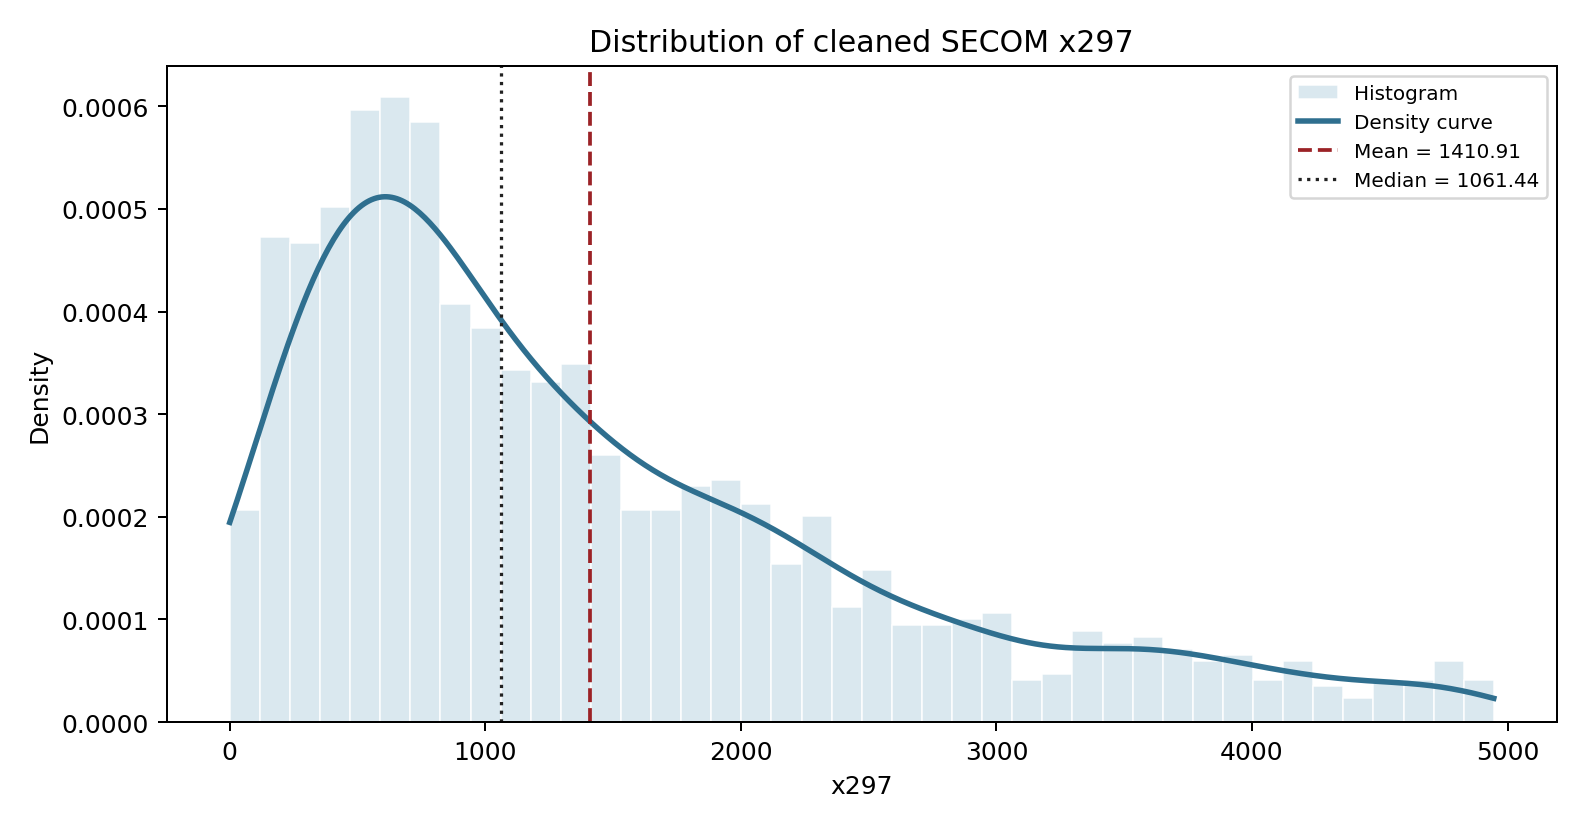
\includegraphics[width=0.7\linewidth]{variable_distribution_x297.png}
    \end{figure}
\end{frame}

%================================================
\begin{frame}{Phase I / Phase II Split}
\[
    m = \lfloor 0.5n \rfloor = \lfloor 0.5(1437) \rfloor = 718
\]
    \begin{table}
        \centering
        \begin{tabular}{lrr}
            \toprule
            Phase & samples & Mean / SD \\
            \midrule
            Phase I & 718 & 1403.64 / 1105.53 \\
            Phase II & 719 & 1418.18 / 1147.80 \\
            \bottomrule
        \end{tabular}
    \end{table}
    \begin{itemize}
        \item Phase I is used as the in-control reference sample
        \item Phase II is monitored sequentially using the chart limits estimated from Phase I
    \end{itemize}
\end{frame}

%================================================
\begin{frame}{Cleaned Series and Phase Split}
\centering
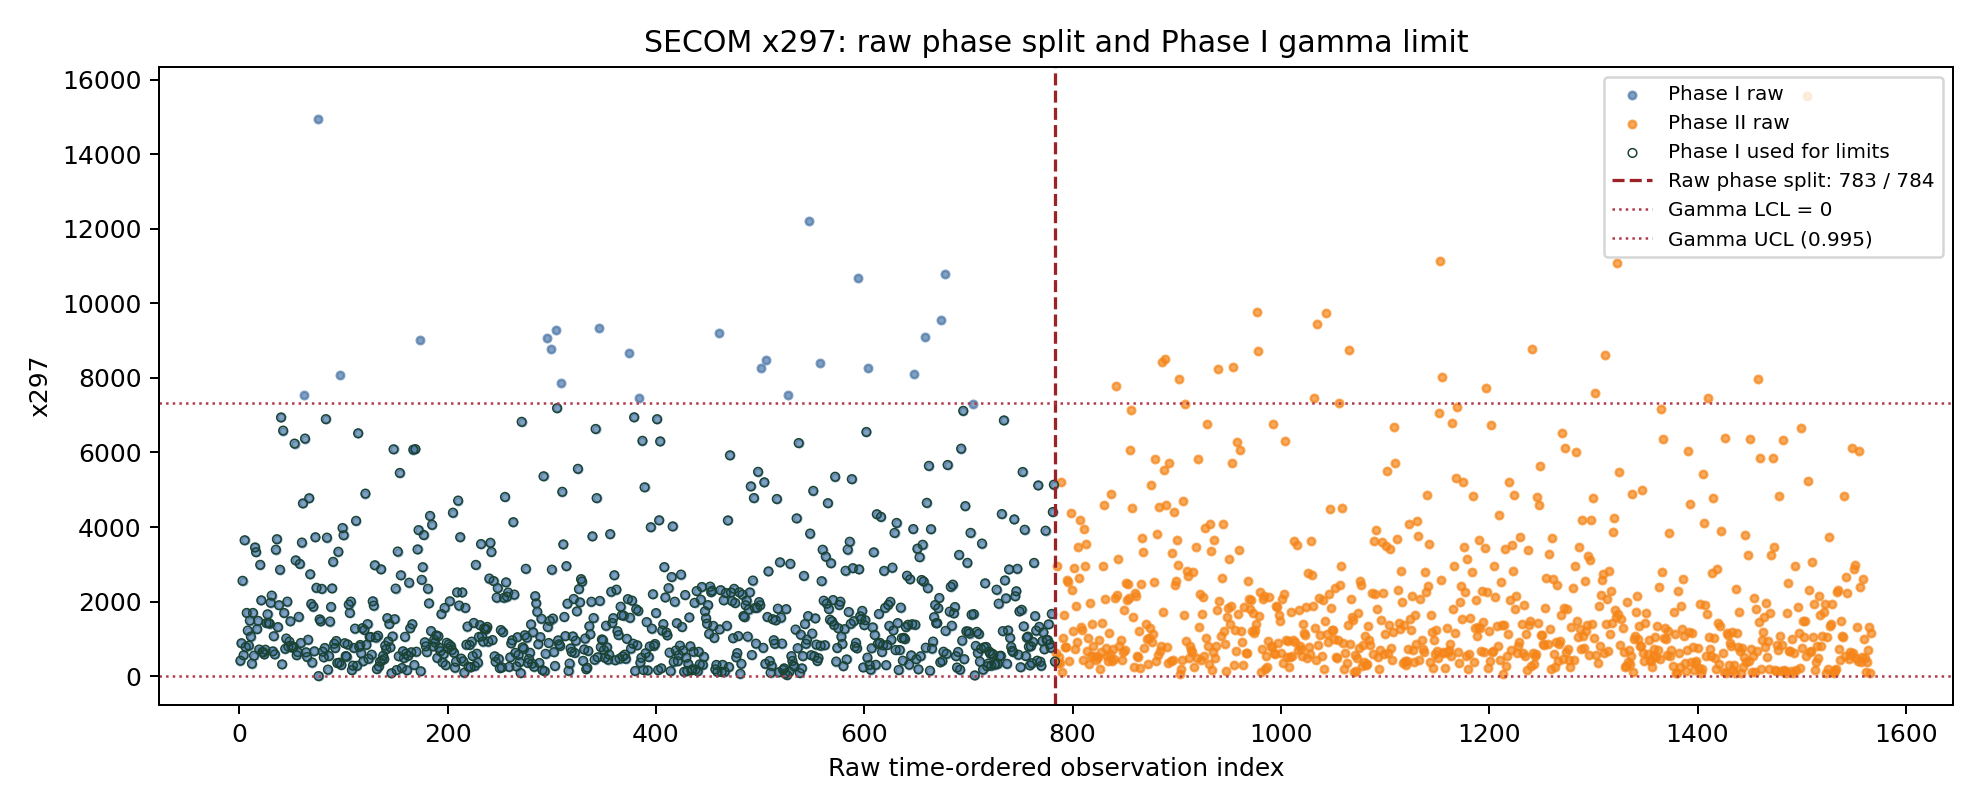
\includegraphics[width=0.94\linewidth]{series_phase_split.png}
\end{frame}

%================================================
\begin{frame}{Phase I RS/P Diagnosis}
\begin{block}{Recursive Segmentation + Permutation Calibration}
\[
    p_{\text{level}} = 0.8675,\quad
    p_{\text{scale}} = 0.8325
\]
\end{block}

% \item Phase I RS/P diagnosis does not reject stability, so the reference sample is usable.

\begin{itemize}
    \item Phase I shows no signifacant evidence of level or scale change
    \item Phase I data can be regarded as stable
\end{itemize}
\end{frame}

%================================================
\begin{frame}{Chart Design}
\begin{table}
\centering
\scriptsize
\begin{tabular}{p{0.28\linewidth}p{0.17\linewidth}p{0.42\linewidth}}
\toprule
Method & Target & Main setting \\
\midrule
Individuals Shewhart & Mean & 3-sigma limits \\
Mean EWMA & Mean & $\lambda=0.1,\ \rho=2.454$ \\
Variance EWMA & Variance & $\lambda=0.1,\ \rho_U=2.595,\ \rho_L=1.580$ \\
Adaptive EWMA & Mean & \makecell[l]{\(\eta_1(e_n)\): \(\mu_1=1,\ \mu_2=4,\ ARL_0=100\),\\
                        \(h=0.7874,\ \lambda=0.1813,\ u=2.5752\)} \\
Mean CUSUM & Mean & $k=0.5,\ h=4.095$ \\
Variance CUSUM & Variance & $k_U=1.848,\ h_U=7.416$; $k_L=0.462,\ h_L=-2.446$ \\
CPD charts & Mean / variance / joint & $\alpha=0.005$ \\
\bottomrule
\end{tabular}
\end{table}

\end{frame}

%================================================
\begin{frame}{Mean-Shift Monitoring Results {\small (Main Mean Charts)}}
    \scriptsize
    \begin{columns}[T,totalwidth=\linewidth]
        % 左欄：文字結果
        \begin{column}{0.3\linewidth}
            \normalsize
            \centering
            \vspace{0.3cm}
            \textbf{Mean EWMA}\\
            First signal: 743\\
            Signal count: 17

            \vspace{0.8cm}
            \textbf{Adaptive EWMA}\\
            First signal: 743\\
            Signal count: 32

            \vspace{1cm}
            \textbf{Mean CUSUM}\\
            First signal: 743\\
            Signal count: 13
        \end{column}
        
        % EWMA、AEWMA 與 CUSUM 皆於 743 發出訊號

        % 右欄：三張圖
        \hspace{1.5em}
        \begin{column}{0.8\linewidth}
            \vspace{-0.5em}
            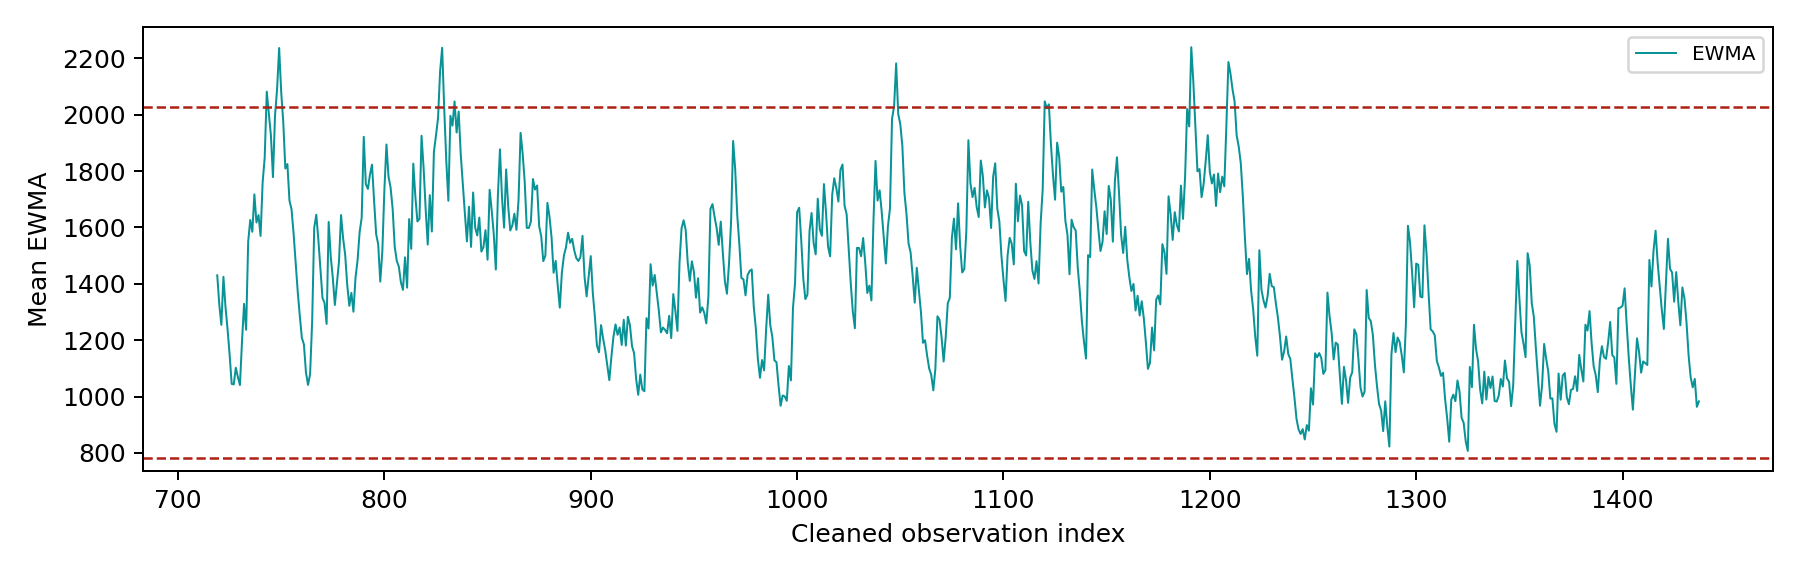
\includegraphics[width=0.65\linewidth]{mean_ewma.png}\\[-0.4em]
            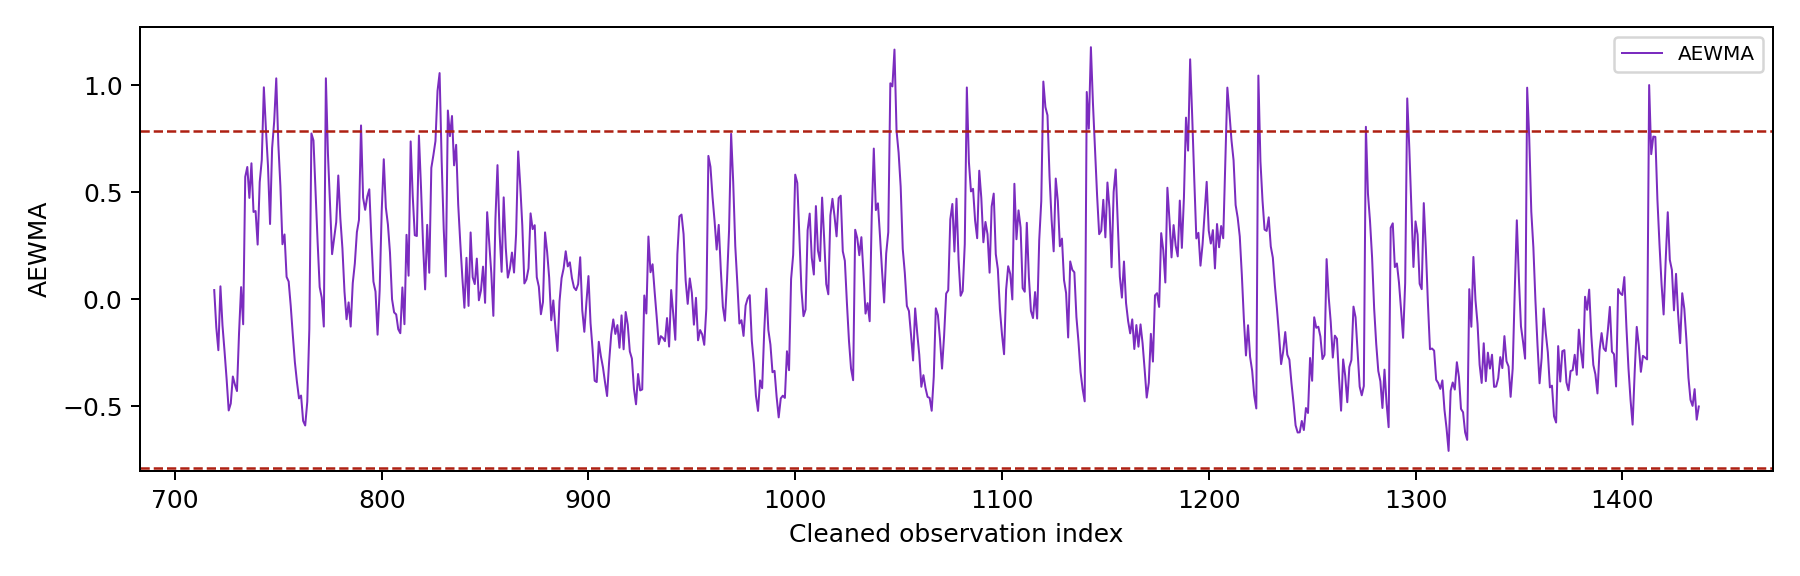
\includegraphics[width=0.65\linewidth]{adaptive_ewma.png}\\[-0.4em]
            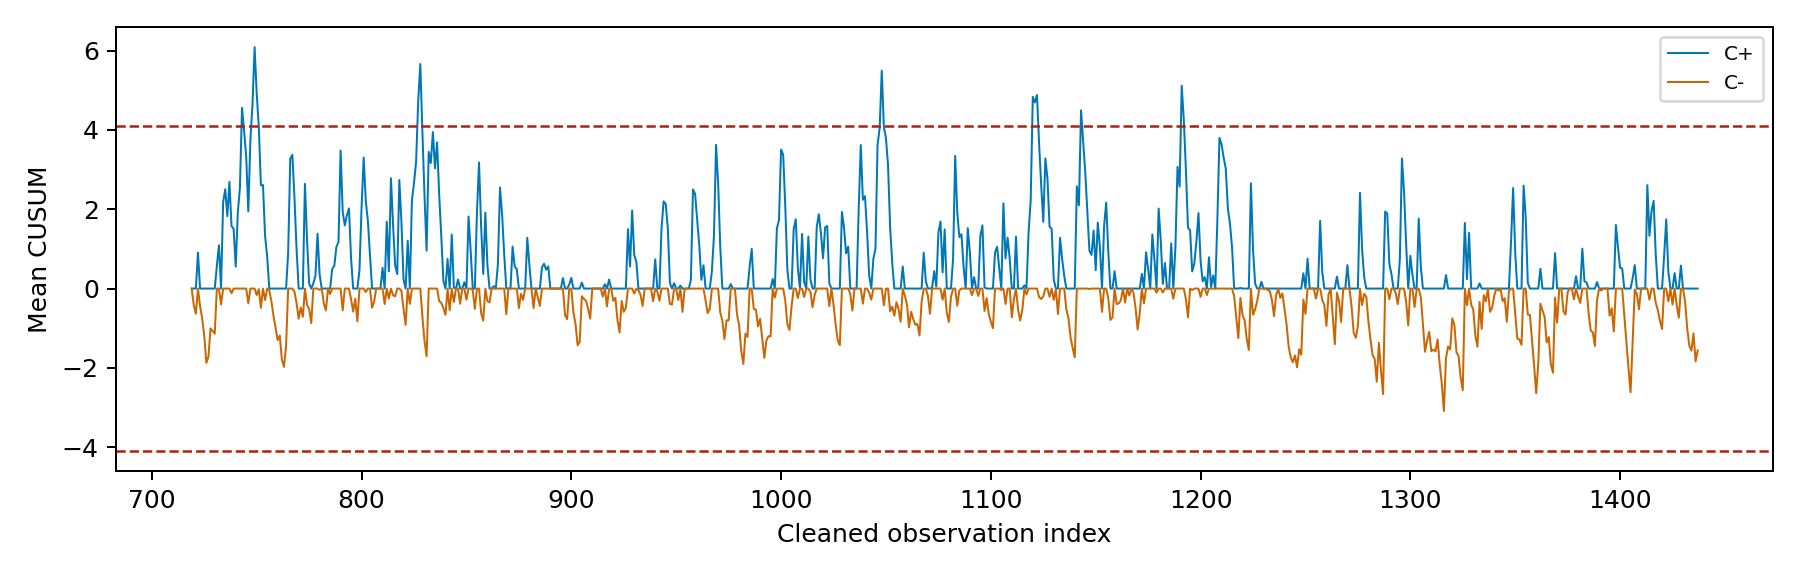
\includegraphics[width=0.65\linewidth]{mean_cusum.png}
        \end{column}
    \end{columns}
\end{frame}

%================================================

\begin{frame}{Mean-Shift Monitoring Results {\small (Supplementary Charts)}}
    \begin{columns}[T,totalwidth=\linewidth]
        % 左欄：文字結果
        \begin{column}{0.25\linewidth}
            \centering
            \vspace{0.3cm}
            \textbf{Individuals Shewhart}\\
            First signal: 773\\
            Signal count: 10

            \vspace{1.5cm}
            \textbf{CPD Mean}\\
            First signal: 749\\
            Signal count: 118
        \end{column}

        % Shewhart 較晚，CPD mean chart 則顯示較高的訊號頻率

        % 右欄：二張圖
        \hspace{1em}
        \begin{column}{1.1\linewidth}
            \vspace{-0.5em}
            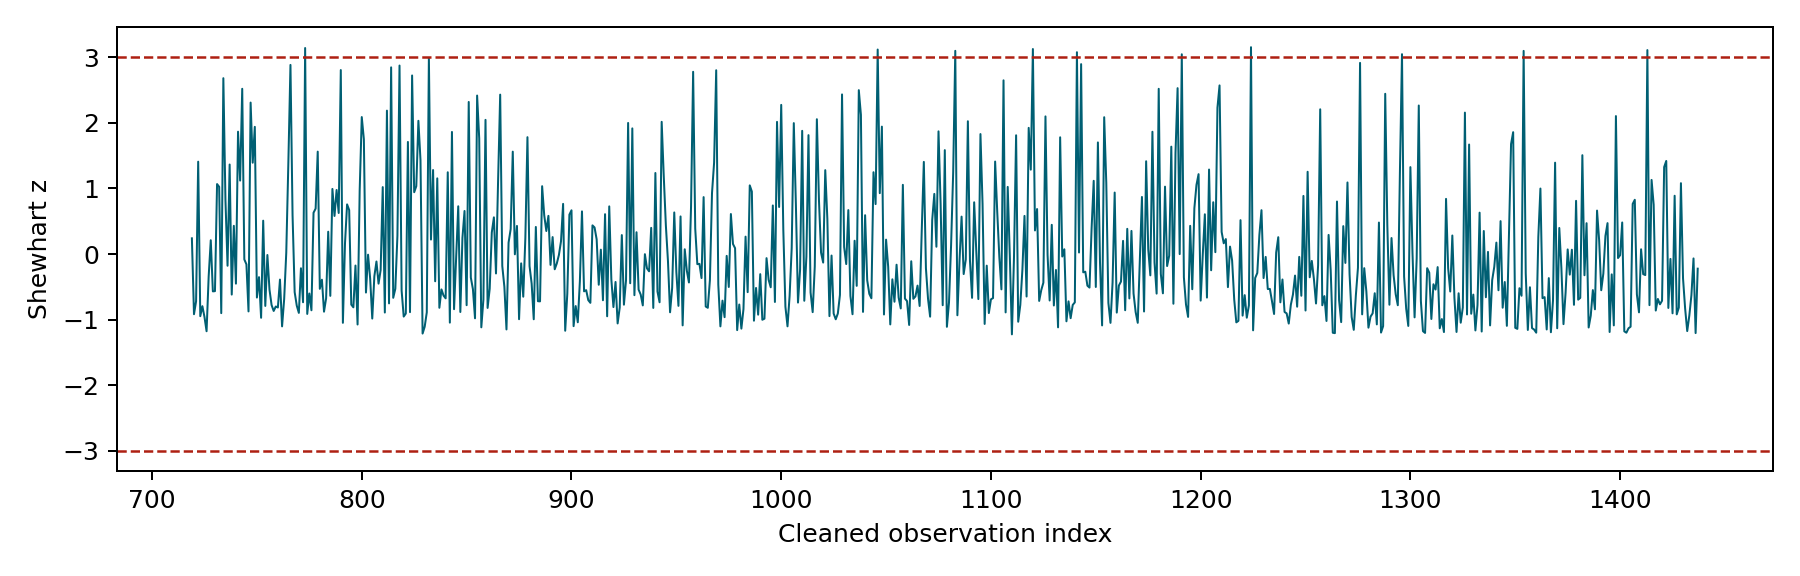
\includegraphics[width=0.65\linewidth]{mean_shewhart.png}\\[-0.4em]
            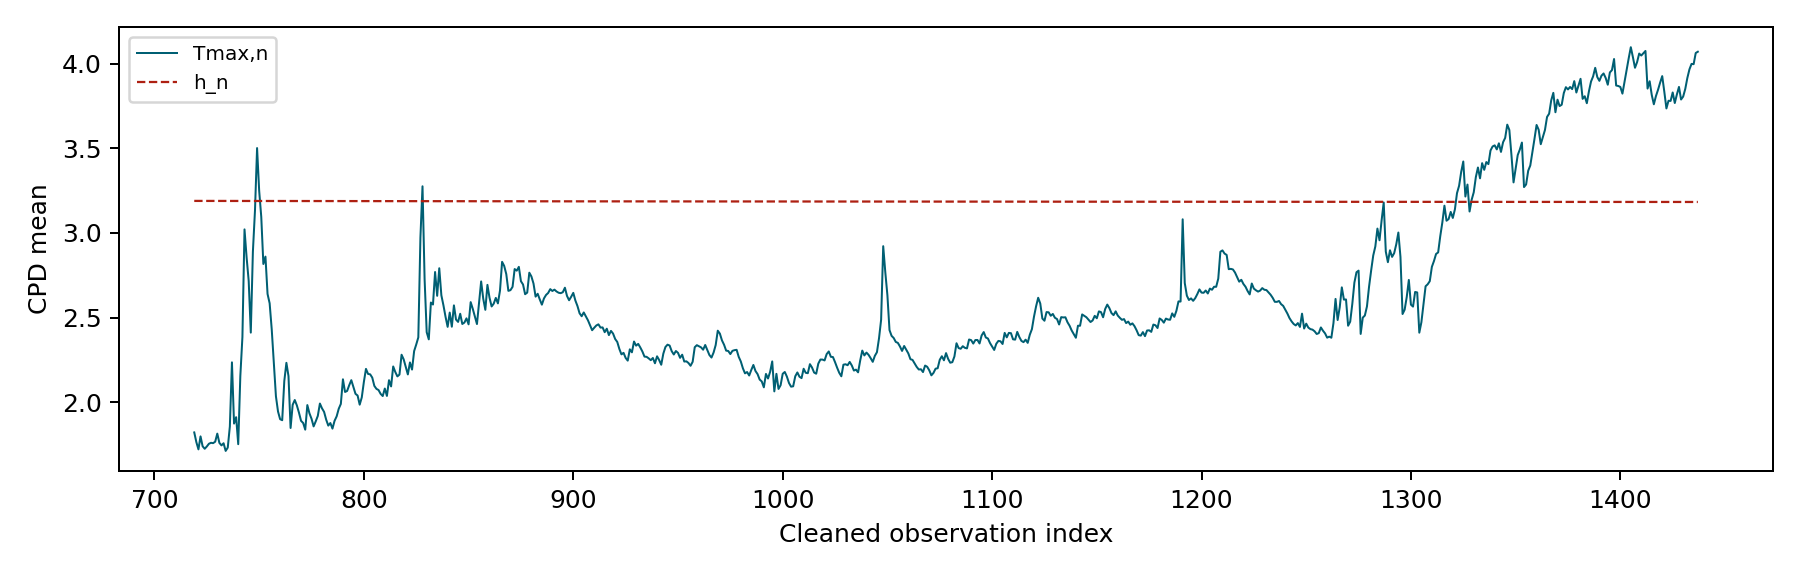
\includegraphics[width=0.65\linewidth]{cpd_mean.png}\\[-0.4em]
        \end{column}
    \end{columns}
\end{frame}

%================================================
\begin{frame}{Variance-Shift Monitoring Results {\small (Target: Variance)}}
    \begin{columns}[T,totalwidth=\linewidth]
        % 左欄：文字結果
        \begin{column}{0.25\linewidth}
            \centering
            \vspace{0.5cm}
            \textbf{Variance EWMA}\\
            First signal: 719\\
            Signal count: 719

            % \item Variance-sensitive methods are more aggressive, especially variance EWMA.

            \vspace{1.8cm}
            \textbf{Variance CUSUM}\\
            First signal: 773\\
            Signal count: 59
        \end{column}
        
        % Variance EWMA 於 Phase II 第一筆觀測即發出訊號
        
        % 表示變異數偏移是最早出現的異常型態。

        % 右欄：二張圖
        \hspace{1em}
        \begin{column}{1.1\linewidth}
            \vspace{-0.5em}
            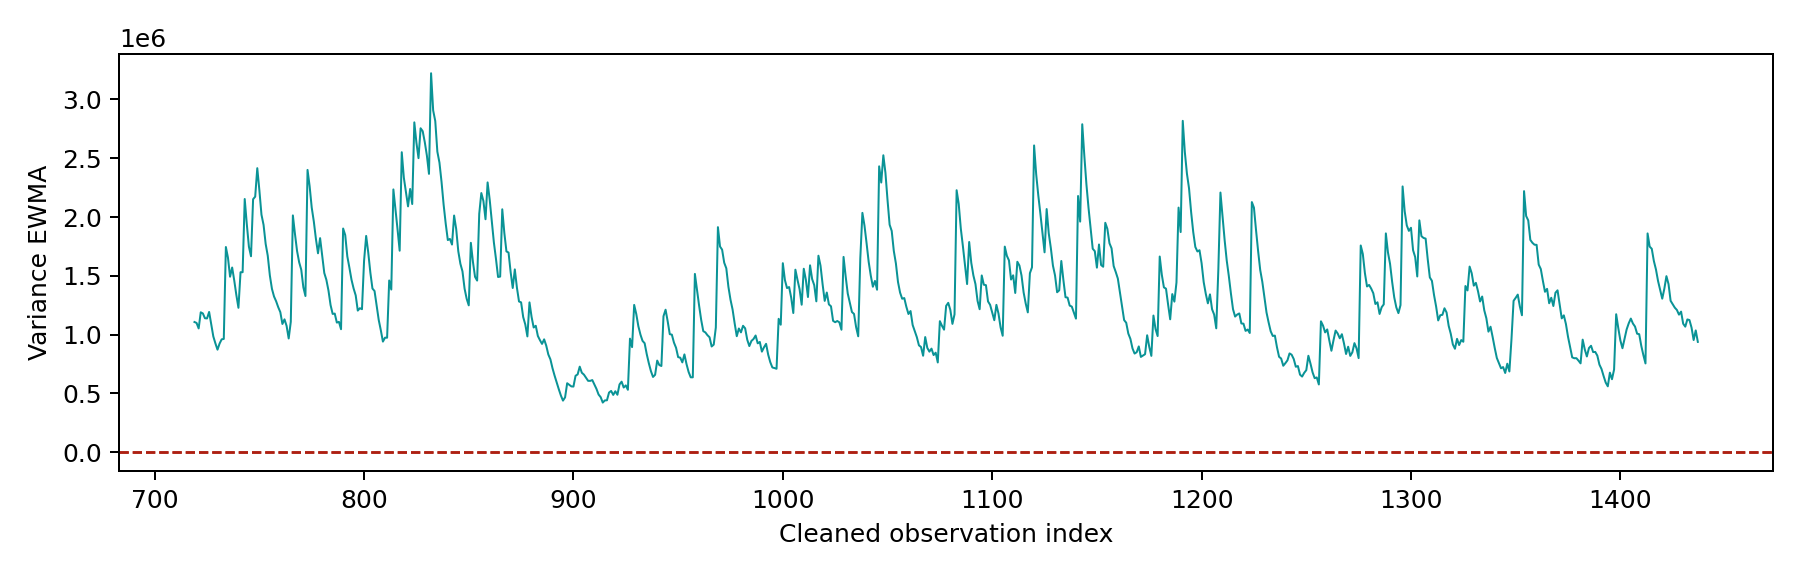
\includegraphics[width=0.65\linewidth]{variance_ewma.png}\\[-0.4em]
            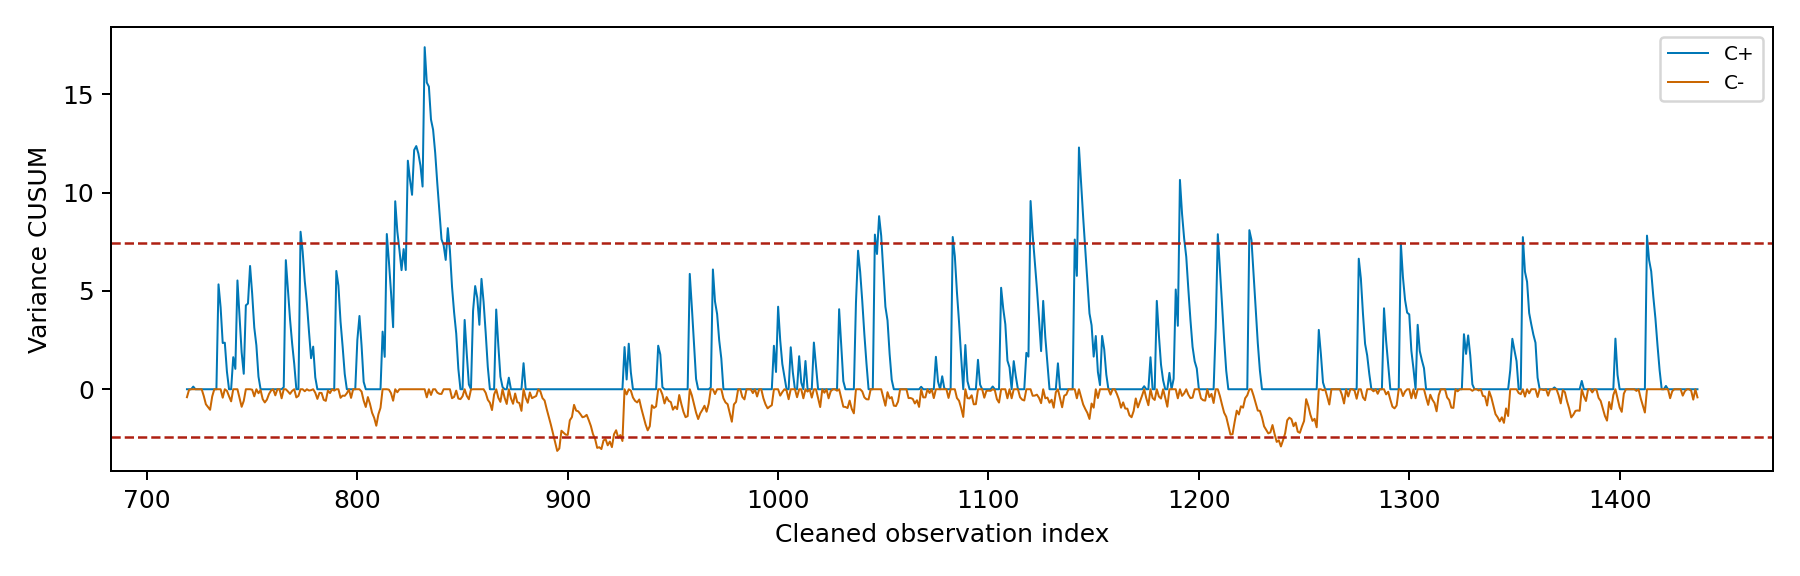
\includegraphics[width=0.65\linewidth]{variance_cusum.png}\\[-0.4em]
        \end{column}
    \end{columns}
\end{frame}

%================================================

\begin{frame}{CPD and Joint Monitoring Results}
    \begin{columns}[T,totalwidth=\linewidth]
        % 左欄：文字結果
        \begin{column}{0.25\linewidth}
            \centering
            \vspace{0.5cm}
            \textbf{CPD joint}\\
            First signal: 762\\
            Signal count: 71

            \vspace{1.8cm}
            \textbf{CPD variance}\\
            First signal: 761\\
            Signal count: 78
        \end{column}

        % CPD variance 與 CPD joint chart 的訊號時間接近
        
        % 表示製程可能同時存在變異數改變與結構性變化

        % 右欄：二張圖
        \hspace{1em}
        \begin{column}{1.1\linewidth}
            \vspace{-0.5em}
            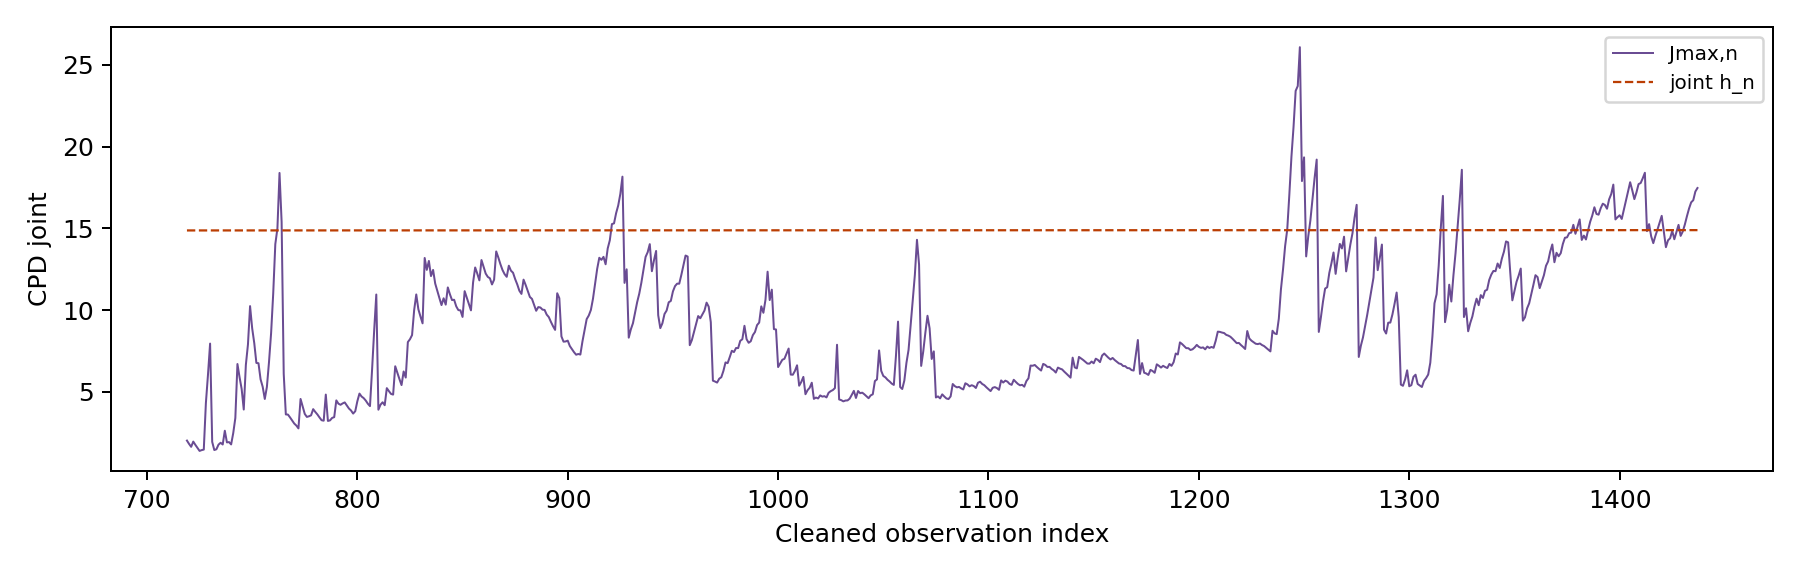
\includegraphics[width=0.65\linewidth]{cpd_joint.png}\\[-0.4em]
            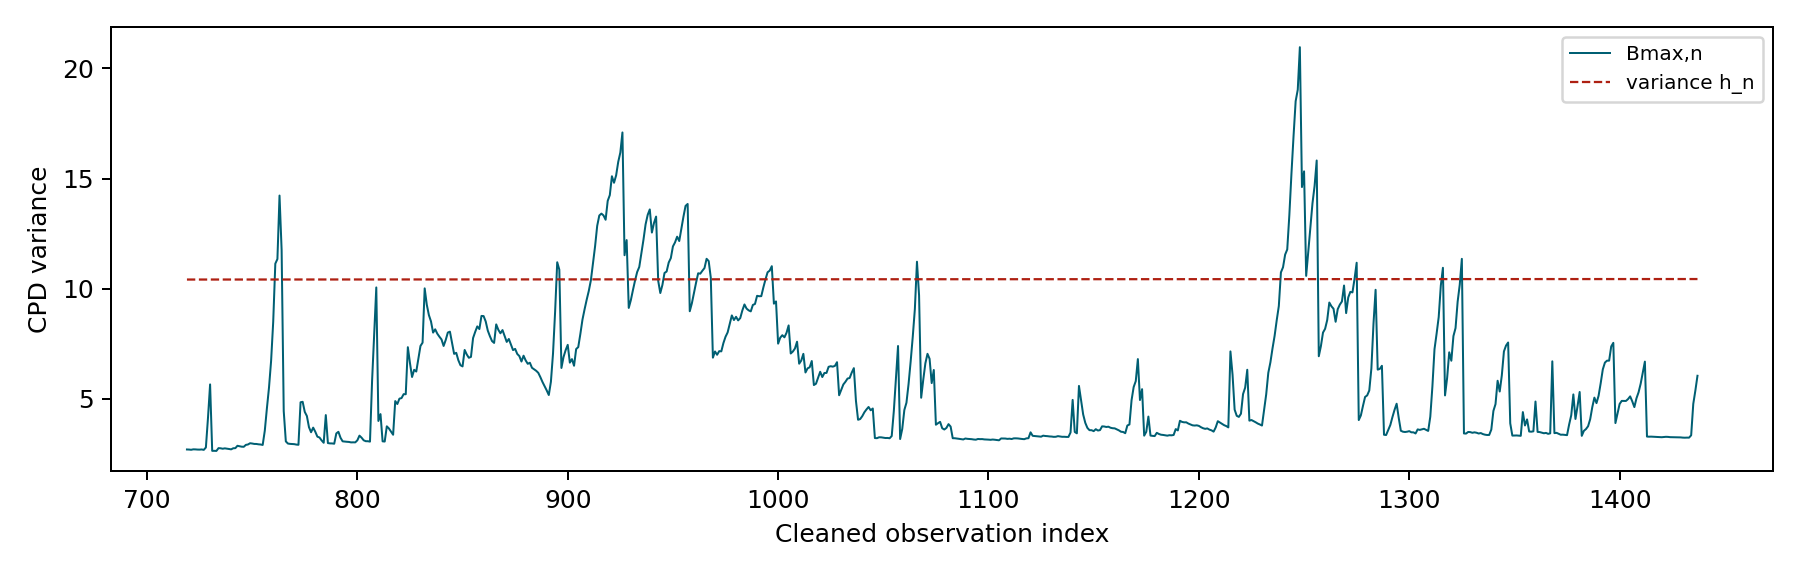
\includegraphics[width=0.65\linewidth]{cpd_variance.png}\\[-0.4em]
        \end{column}
    \end{columns}

% The earliest signal is produced by the variance EWMA chart at index 719,
% suggesting that the process change first appears as a variance shift.
% Mean-sensitive charts later signal at index 743, indicating that a mean shift
% also emerges after the initial variance instability.
% CPD-based charts further suggest persistent structural changes in Phase II.

\end{frame}

%================================================

\begin{frame}{CPD Post-Signal Interpretation}
    \begin{itemize}
        \item The strongest CPD mean signal estimates:
        \[
            \widehat{r} \approx 1212
        \]
        \item The strongest CPD variance and joint signals estimate:
        \[
            \widehat{r} \approx 1229
        \]
    \end{itemize}

    % \item CPD variance and joint charts locate later structural changes around indices 1229.

\end{frame}

%================================================
\begin{frame}{Conclusion}
\begin{enumerate}
    \item The selected SECOM variable $x_{297}$ is usable
    \vspace{0.5em}
    \item Phase I RS/P results support using the first 718 samples as the IC reference
    \vspace{0.5em}
    \item The variance EWMA is very sensitive
    \vspace{0.5em}
    \item CPD charts suggest structural changes around indices 1212--1229
\end{enumerate}
\end{frame}

\end{document}
